\documentclass[aps,prl,reprint,superscriptaddress]{revtex4-1}

%--- PACKAGES ---%
% \usepackage[T1]{fontenc}
\usepackage{graphicx}
\usepackage[usenames,dvipsnames]{color}
\usepackage{amsmath,amssymb}
\usepackage{bm}
\usepackage{upgreek}
\usepackage{xspace}
\usepackage{units}
\usepackage{hhline}
\usepackage[vskip=0pt]{quoting}
\usepackage[colorlinks,urlcolor=blue,citecolor=blue,linkcolor=blue]{hyperref}
\graphicspath{{figures/}}
\renewcommand{\arraystretch}{1.5}

%--- TEXT SHORTCUTS ---%
\newcommand{\etal}{et~al.\xspace}
\newcommand{\Rb}{$^{87}$Rb\xspace}
\newcommand{\qmagic}{q_{\text{magic}}\xspace}
\newcommand{\qRmagic}{q_{R,\text{magic}}\xspace}
% \newcommand{\lundblad}{Phys. Rev. Lett. \textbf{118}, 2xxxxx (2017)}
\newcommand{\lundblad}{arXiv:1706.xxxx}

%--- TEXT OPERATORS ---%
\newcommand{\reffig}[1]{\mbox{Fig.~\ref{#1}}}
\newcommand{\refeq}[1]{\mbox{Eq.~(\ref{#1})}}
\newcommand{\refsec}[1]{\mbox{Sec.~(\ref{#1})}}
\newcommand{\note}[1]{\textcolor{ForestGreen}{[\textrm{#1}]}} % Make editorial notes red

%--- MATH OPERATORS ---%
\newcommand{\upd}{\text{d}}
\newcommand{\totalD}[2]{\frac{\upd #1}{\upd #2}}
\newcommand{\partialD}[2]{\frac{\partial #1}{\partial #2}}
\newcommand{\vecop}[1]{\hat{\mathbf{#1}}\xspace}
\newcommand{\expect}[1]{\langle #1 \rangle}
\newcommand{\abs}[1]{\vert #1 \vert \xspace}
\newcommand{\bra}[1]{\langle #1 \vert \xspace}
\newcommand{\ket}[1]{\vert #1 \rangle \xspace}
\newcommand{\braket}[2]{\langle #1 \vert #2 \rangle \xspace}
\newcommand{\vect}[1]{\mathbf{#1}\xspace}
\newcommand{\uvect}[1]{\hat{\mathbf{#1}}\xspace}
\newcommand{\epvec}{\hat{\mathbf{\epsilon}}\xspace}
\newcommand{\jvect}{\mathbf{\tilde{E}}\xspace}
\newcommand{\ham}{\mathcal{H}}

% Underscores in text (from http://tex.stackexchange.com/a/38720)
\catcode`_=12
\begingroup\lccode`~=`_\lowercase{\endgroup\let~\sb}

\begin{document}

\title{Continuously observing the spectrum of a dynamically decoupled spin-1 quantum gas}

\author{R.\,P.~Anderson}
\author{M.\,J.~Kewming}
\author{L.\,D.~Turner}
\affiliation{School of Physics \& Astronomy, Monash University, Victoria 3800, Australia.}

\date{\today}

\begin{abstract}
Quantum systems can be engineered so that their spectra are sensitive to a particular measurand whilst simultaneously impervious to parasitic fluctuations of an environment.
Here we use a minimally perturbative atom-light interface to study the dressed-state energy spectrum of a spin-1 quantum gas continuously and in-situ.
The spins are coupled by a radio-frequency field, whose amplitude sets the frequency band in which oscillating magnetic fields manifest a linear measurand, and we probe the energy spectrum while the system evolves unitarily.
By varying a symmetry-breaking parameter of the Hamiltonian, we find a regime in which two of the dressed states are maximally insensitive (up to fourth-order) in magnetic field fluctuations that are slow compared to the dressed-state splittings.
Moreover, we demonstrate the predictive power of our continuous probe to tune the measurement band and optimize the dynamical decoupling.
This robust system shares the useful hallmarks of quantum metrology platforms; the states are thus termed ``psuedo-clock'' states in a co-published result by Lundblad~\emph{et al.} (Phys. Rev. Lett. \textbf{118}, 2xxxxx (2017)) and are candidates for band-tunable magnetometry and color charge analogues in quantum gases. 
\end{abstract}

\maketitle

\section{Introduction}
\label{sec:introduction}
\begin{itemize}
    \item Minimally insensitive states in other systems, e.g. $\ket{F=1,m=-1} \leftrightarrow \ket{F=2,m=+1}$ at $B=3.23\unit{G}$, and variants thereof (including those insensitive to Rabi frequency variations reported on at Otago in 2016).
\end{itemize}

\begin{figure}
    \centering
    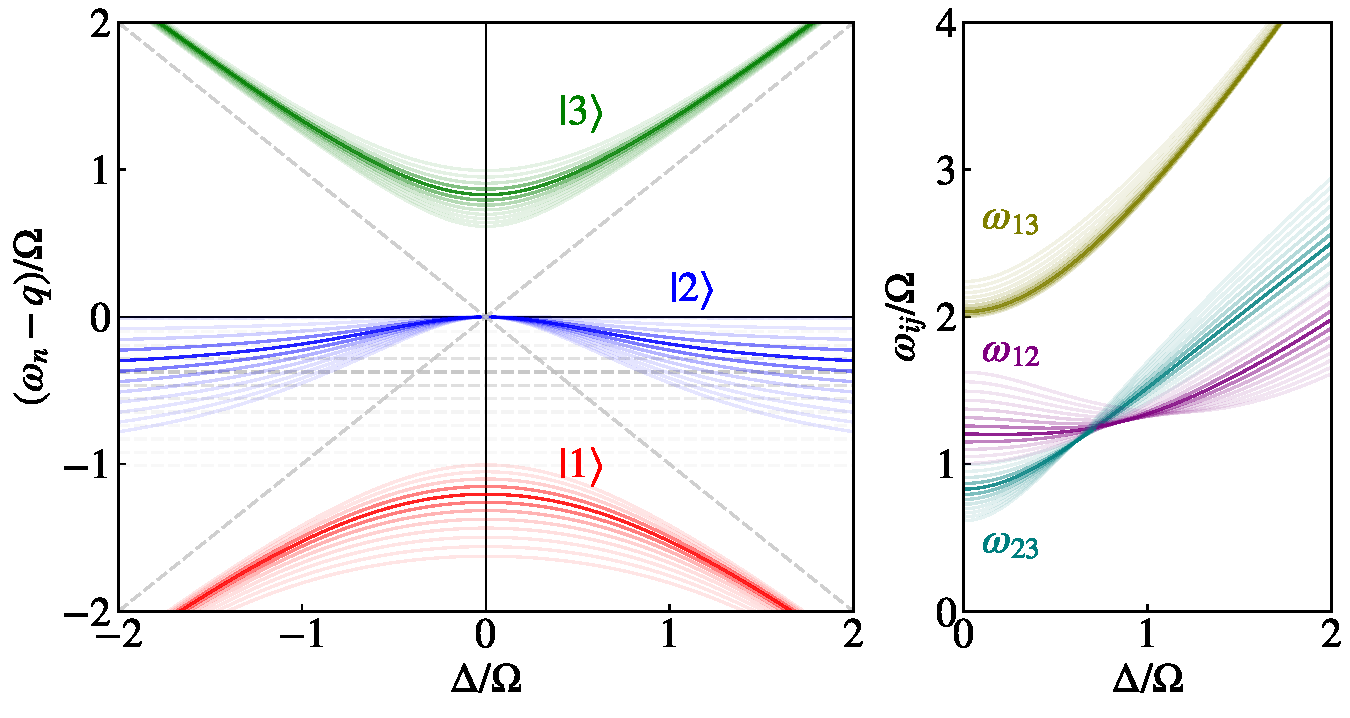
\includegraphics[width=\columnwidth]{figure_1.pdf}
    \caption{
    \label{fig:eigensystem_schematic}
        (Color online)
        Energy spectrum and splittings of a radiofrequency coupled spin-1 for various $q(B)\in[0,\Omega]$.
        The transparency and thickness of each curve is proportional to the distance of the quadratic shift $q$ from $\qmagic\approx 0.348\Omega$.
        (Left) Energies $\omega_n$ of dressed states $\ket{n}=\ket{1}$, (red) $\ket{2}$ (blue), and $\ket{3}$ (green) normalized to the rf-coupling strength (Rabi frequency) $\Omega$ as a function of detuning $\Delta(B)=\omega_{\text{rf}}-\omega_L(B)$,
        Dashed lines indicate the energies of uncoupled states ($\Omega=0$) in a frame rotating at $\omega_{\text{rf}}$.
        (Right) Splittings $\omega_{ij}$ of dressed states $\ket{i}$ and $\ket{j}$ as a function of detuning.
        When $q=\qmagic$, energies $\omega_1$ and $\omega_2$ share the same curvature, and their difference $\omega_{12}$ (right, purple) is minimally sensitive to detuning and thus magnetic field variations. 
    }
\end{figure}



\bibliography{dressed_faraday}
   
\end{document}